\section{RethinkDB}
\chapterauthor{Anne Born, Dorian Czichotzki}

\subsection{Introduction}
In today's data-driven world, the availability of information in real-time becomes more and more important. Many applications rely on an analysis and delivery of data in a time-frame that is considered as immediate by the user. Be it multi-player games, real-time analytics or connected devices in an IoT infrastructure \autocite{Wingerath2017}. Data should not only be delivered quickly but also proactively, focusing more on a push-based architecture, giving the responsibility to keep the client informed to the server, instead of the conventional pull-based database were the client has to request information each time it is of interest.  One kind of technology, implementing this immediate handling of information are so called real-time databases, which are discussed in this chapter by reference to RethinkDB, an example for such a push-based database.
The chapter is structured as follows.


First, an introduction to real-time databases in general is provided and a concrete definition of the term in the context of RethinkDB is given. The following sections then discusses the real-time database RethinkDB in great detail, providing information on the architecture, use-cases it is suited for, and most importantly where the technology could be placed in the CAP-Theorem.

\subsection{Real-time Databases}
\label{sec:rethink_real-time}
Like many terms in the IT, real-time databases have an abundance of different definitions. Some overlapping to a great extend, others having nearly no intersection at all. This makes for a need to introduce some of the most common definitions with the goal of establishing a precise interpretation of the term in the context of this book and - particularly - this chapter.


One of the first indications of the term real-time database was within a special issue of the ACM SIGMOD Record on Real-Time Database Systems in March 1988 \autocite{Eich:1988:44203}. In an article of this journal called "Issues and Approaches to Design of Real-Time Database Systems" Mukesh Singhal defined the use-case for real-time databases as "applications which have severe performance constraints such as fast response time and continued operation in the face of catastrophic failures" \autocite[p.  1]{Singhal:1988:IAD:44203.44205}. He further mentions timing constraints as a direct derivation of the use-cases mentioned above, laying a fundamental basis for one of the most common definitions of said technology.


This definition (referring to real-time databases as databases that fulfil time-constraints and must meet certain deadlines), also probably the most popular one, is not the one used in the context of RethinkDB.


Instead, the definition used in this book is based on a medium article by Wolfram Wingerath \autocite{Wingerath2017} who claims that "in recent years, people have come to expect reactivity from their applications, i.e. they assume that changes made by other users are immediately reflected in the interfaces they are using" \autocite{Wingerath2017}. From this statement it can already be derived that he defines the use-cases for real-time databases differently from Singhal. Instead of applications that need fast response time for security reasons, like applications for power-plants or hospitals, he defines a general demand for reactive applications for the sole reason of improved user experience. However, similarly to Singhal, Wingerath also sees a need for new technology besides conventional databases. Conventional databases being pull-based applications that only represent the state of the system at a single point in time. As an alternative to those databases he defines real-time databases as technology that facilitates the push-based handling of changes, "taking view maintenance out of the application layer" \autocite{Wingerath2017}. A real-time databases thus must provide some functionality for clients to 'subscribe' to certain events (changes), receiving updates when the event is triggered. This subscription-feature' is what he calls 'real-time queries'.


Real-time queries can fall into one of two different categories:

\begin{itemize}
    \item Self maintaining queries
    \item Event stream queries
\end{itemize}

The former delivers not only the information that something has changed but also the old and new value. This of course only works if the query is executed again each time a change took place. The latter type of queries only provides the information that a change took place without any more details.


Both queries are push based, pushing information to the client.


Summarised, real-time databases, as defined in this book, are databases that facilitate a push-based method instead of only allowing pull-based query execution. This makes the development of reactive applications much more feasible, since it allows for data updates in a publish/subscribe-like manner.

\subsection{RethinkDB}
After giving an introduction to real-time databases as defined in this book, the document-based database RethinkDB is introduced and discussed in great detail. In order to understand not only the database itself but also its place in the CAP-Theorem this chapter is structured in the following sections: Firstly this section will provide an overview over RethinkDB and its core features, next a short section on the history of the database gives some more insight into the story of RethinkDB and its community, then the proprietary query language ReQL is introduced and explained briefly. Finally the architecture that this database is based on is outlined, including the distribution of RethinkDB over multiple nodes, the functioning of query executions and the storing of data.


Most of the information displayed in this chapter is from the official RethinkDB website \autocite{rethinkdb}.\bigskip
RethinkDB defines itself as "the open-source database for the real-time web" \autocite{rethinkdb}.


From this description it is already possible to derive two of the most important features of the database project. The first being that it is 'open-source' meaning that its source code is publicly available\footnote{https://github.com/rethinkdb/rethinkdb}. RethinkDB itself is developed and enhanced by a combination of core team developers and database experts as well as over 100000 other contributors from the RethinkDB community, using the open-source aspect to provide their knowledge to the project.


The second feature that the RethinkDB project uses frequently to describe itself is being a database 'for the real-time web'. This means, that RethinkDB falls exactly in the definition of real-time databases established in \autoref{sec:rethink_real-time}, providing a function called "changefeeds" (see \autoref{sec:rethink_changefeeds}) that is push-based and thus automatically updates the client in case of changes.


This feature is already a pretty unique characteristic of RethinkDB.
Another one is the fact that the ambitious project was written from the ground up in C++, not relying on and extending existing database implementations.
This approach of creating something completely new and \enquote{rethinking} databases also lead to the development of a proprietary querying language, that is discussed in \autoref{sec:rethink_reql}.

\subsubsection{History}
RethinkDB is originally the product of the eponymous company founded in 2009 with the goal to "bring a breath of fresh air to the database world" \autocite{rethinkdb:announcement}. At this point the database was not open-source, but also not released as a production ready version yet. With version 1.2 released in November 2012, the company first decided to open-source their project \autocite{rethinkdb:open_source}.


After three more years of development in 2015, RethinkDB 2.0 was released and with it the first production ready version of the real-time database \autocite{rethinkdb:production_ready}. One year later, however, the company was shut down, terminating the official support for the production versions that was offered until then \autocite{rethinkdb:shutting_down}. In the blog article announcing the shut down of the company, it was also signalised that the RethinkDB team plans on continuing the development of their product with an open-source continuity plan, keeping it available under an open-source license. Due to this continuous effort of former RethinkDB employees and people from the community to "transition it to a community-driven endeavour" \autocite{rethinkdb:linux_foundation}, the source-code was purchased by the Cloud Native Computing Foundation in 2017, who published it under the Apache License 2.0.


As of today the RethinkB project is extended by a large open-source community with version 2.3 being the latest release.

\subsubsection{ReQL}
\label{sec:rethink_reql}

As mentioned previously, one of the main features of RethinkDB is its powerful, proprietary query language called ReQL.
Since this language is the base of all interaction between the client and the server (the database), it will be discussed in detail in the following sections, explaining its core attributes, the supported data-types and providing examples for different functionalities \autocite{rethinkdb_reql}.

\paragraph{Data Types}
To facilitate a deeper understanding of ReQLs mechanics, this section gives an insight into the different data types that are supported by the querying language.
In the official documentation, RethinkDB distinguishes two main categories \autocite{rethinkdb:data_types}:

\begin{itemize}
    \item Basic data types
    \item RethinkDB-specific data types
\end{itemize}

Each of the aforementioned categories is explained briefly.

\subparagraph{Basic data types}
This category includes the data types supported by nearly every programming or query language.

\begin{itemize}
    \item Numbers
    \begin{itemize}
        \item This data type includes any real number. Internally values of this type are represented as double precision floating point numbers. This leads to a size of 64 bits.
        \item allowed (examples): 2, 5.8276, -13.4
        \item not allowed: infinity, NaN
    \end{itemize}
    \item Strings
    \begin{itemize}
        \item The data type of string is used the same way it is commonly used in other query languages as well. The encoding used by ReQL is UTF-8, which is why any valid UTF-8 string is also a valid ReQL string. This includes the usage of the null code point (U+0000).
    \end{itemize}
    \item Booleans
    \begin{itemize}
        \item A boolean can attain the values true or false.
    \end{itemize}
    \item Null
    \begin{itemize}
        \item Nearly every programming language has a data type similar to Null, however the naming may be different from language to language. Since ReQL can be embedded into many different programming languages (see \ref{sec:rethink_reql_features}) it might be called something different from Null (e.g.: nil or none). It is important to mention that Null does not equal the number zero (0), the empty set ({}) or a string with a length of zero (""). Instead Null is used to emphasise the absence of a value. For example the parent of a root node could be Null, since it does not exist.
    \end{itemize}
    \item Objects
    \begin{itemize}
        \item Since RethinkDB belongs to the category of document stores and it more specifically is designed to  store JSON documents, any valid JSON object is also a valid object in ReQL. This includes but is not limited to simple key-value pairs \textit{({name: "Harry Potter"})} or nested objects. 
    \end{itemize}
    \item Arrays
    \begin{itemize}
        \item Equally to the documents mentioned above, the array data type of ReQL is also based on JSON arrays, meaning that any valid JSON array is also a valid ReQL array \textit{([1, 2, 3] [] [{name: 'Harry', age: 23}, {wizard: 'Dumbledore', age: 112}])}. The maximum number of elements inside an array can be changed at runtime, the default, however, is 100000. But RethinkDBs internal handling of arrays makes them inefficient at large sizes
    \end{itemize}
\end{itemize}

\subparagraph{RethinkDB-specific data types}
Data types of this category are specific to the functioning of RethinkDB and ReQL. They are not supposed to be used as actual data but instead are either what RethinkDB uses internally to store data or as return values to queries. An exception to this are the so-called 'pseudo types'. Those can be used as actual data types for values defined by the user, but are specific to RethinkDB in a way that they are not commonly implemented in most programming languages.

\begin{itemize}
    \item Databases
    \begin{itemize}
        \item This data type describes RethinkDB databases. When using the '.db' operation, this is the return value. A database holds tables and administrative information.
    \end{itemize}
    \item Tables
    \begin{itemize}
        \item This data type describes RethinkDB tables. They can be used as selectors. Additionally documents can be added, updated or deleted making tables writable.
    \end{itemize}
    \item Streams
    \begin{itemize}
        \item Similar to the aforementioned arrays, streams are lists. However, in order to make working with large result sets more feasible a Stream is represented by a cursor that points to the result set. This means, that instead of retrieving the entire result at once (like an array) a loop is employed to only retrieve one result set at a time, making it more performant. Another difference between streams and arrays is that the former is read-only and thus can not be changed. This limits the chainability of commands that return a stream.
    \end{itemize}
    \item Selections
    \begin{itemize}
        \item Selections are a subset of the table data type. Many table operations (for example \mintinline{python}{filter} and \mintinline{python}{get}) return a selection. Selections exist as a counterpart to three different data types: \mintinline{python}{Selection<Object>}, \mintinline{python}{Selection<Arrays>} and \mintinline{python}{Selection<Stream>}. Due to the chainability of ReQL commands the Selections are writable and can be passed to other ReQL operations
    \end{itemize}
    \item Pseudotypes
    \begin{itemize}
        \item As mentioned previously the pseudotypes form an exception to the other RethinkDB-specific data types since they can be used with user data similarly to the basic types. Generally they are either special cases of other types or a composition of multiple other types. The pseudotypes include binary objects, times and geometry data types.
    \end{itemize}
\end{itemize}

ReQL provides its users with the 'typeOf' command, returning the data type of operations (see \autoref{lst:rethink_typeOf}).

\begin{listing}[ht]
\begin{minted}[breaklines,breakbefore=.]{python}
r.table('wizards').get(1).typeOf()

# returns:
# "SELECTION<OBJECT>"
\end{minted}
\caption{Usage of the TypeOf command}
\label{lst:rethink_typeOf}
\end{listing}

This short description of the data types supported by ReQL already gives an insight to all the possibilities of querying with RethinkDBs proprietary query language. The following sections will extend this insight by introducing some of the many features that ReQL provides.

\paragraph{Features}
\label{sec:rethink_reql_features}

ReQL itself is designed to offer an extensive amount of functionality, enabling users to not only manipulate json documents but also facilitating the usage of common \gls{sql} capabilities. To achieve this ambitious goal the language is based on functional programming languages like Haskell and Lips. However, a knowledge of those languages is not necessary, since ReQL was developed to embed into an abundance of different programming languages. To allow for this natural integration into different languages so called 'drivers' are developed. The official RethinkDB Website groups the existing drivers into three categories:

\begin{enumerate}
    \item Official Drivers
    \begin{itemize}
        \item Drivers developed and maintained by the core team of RethinkDB developers
    \end{itemize}
    \item Community-supported drivers
    \begin{itemize}
        \item Drivers developed and maintained by members of the large open-source community of RethinkDB. To be accepted as a community-supported driver, the json driver protocol has to be used and the features of at least Rethink 2.0 ReQL must be supported.
    \end{itemize}
    \item Drivers with limited features
    \begin{itemize}
        \item Drivers developed by members of the open-source RethinkDB community, that do not provide full support of RethinDB 2.0 ReQL.
    \end{itemize}
\end{enumerate}

A list with all available drivers by category (as of April 2019) can be found in \autoref{appendix:rethinkdb:listofdrivers}.
To use ReQL in one of the (partially) supported programming languages the user must import the driver the way that is specified by said programming language. Afterwards he/she can construct queries by calling methods from the driver.


Listing \autoref{lst:rethink_python_import} shows how this works exemplarily for python. 

\begin{listing}[ht]
\begin{minted}{python}
#import the RethinkDB package
import rethinkdb as r  
#connect to the server on localhost and default port
conn = r.connect()       
#create a table `users`
r.table_create('users').run(conn)  
#get an iterable cursor to the `users` table
r.table("users").run(conn)          
\end{minted}
\caption{Importing ReQL as a package to python}
\label{lst:rethink_python_import}
\end{listing}

 Of course this embedding of ReQL has limitations. One can not use every feature offered by the 'host language'. This applies to those operations, that have side effects and control blocks. Listing \autoref{lst:rethink_side_effects} shows the limitations of embedding ReQL with the help of an example. It illustrates two ways of getting all documents that match certain criteria, one employing operations native to python (if - else) and one employing the 'r.branch' command included in the RethinkDB package.


In this listing only the latter query would work, since the first one is based on python operations with side effects. Other operations and control blocks that can not be used inside ReQL queries include but are not limited to print statements, switch-case statements and loops.

\begin{listing}[ht]
\begin{minted}[breaklines,breakbefore=.]{python}
# WRONG: Get all wizards older than 30 using the `if` statement
r.db("wizards_world").table('wizards').filter(lambda wizard:
    True if wizard['age'] > 30 else False)

# RIGHT: Get all wizards older than 30 using the `r.branch` command
r.db("wizards_world").table('wizards').filter(lambda wizard:
    r.branch(wizard['age'] > 30, True, False))
\end{minted}
\caption{Limitations of the embedding of ReQL}
\label{lst:rethink_side_effects}
\end{listing}

Additionally, this listing also gives an insight into another important functionality of ReQL: Chaining commands. To construct a query in this query language, a nearly arbitrary number of commands can be chained together, separated with '.'.


To emphasise on this feature and to really illustrate how it works, listing \autoref{lst:rethink_chaining} provides a good example for this. First, all documents of a specific table are returned, then by adding '.pluck("last\_name")' only the last\_name field of each document is returned. This can then be filtered further by adding '.distinct()' to it and so forth.
\begin{listing}[ht]
\begin{minted}[breaklines,breakbefore=.]{python}
# Get all entries of a table
r.db("wizard_world").table("wizards")

# Return only the last names of the documents
r.db("wizards_world").table("wizards").pluck("last_name")

# Get all the distinct last names (remove duplicates)
r.db("wizards_world").table("wizards").pluck("last_name").distinct()

# Count the number of distinct last names
r.db("wizard_world").table("wizards").pluck("last_name").distinct().count()
\end{minted}
\caption{Chaining of commands in ReQL}
\label{lst:rethink_chaining}
\end{listing}

As previously mentioned ReQL has many powerful features, including the \gls{sql}-like combination of multiple tables with JOINs. For reasons of performance JOINs in ReQL are automatically distributed (see \nameref{sec:rethink_arch_query_execution}).


Now anyone who is familiar with \gls{sql} knows that many different JOINs exist in the world of databases. RethinkDB supports four, called inner-join, outer-join, eq-join and zip. The first two work similar to their \gls{sql}-counterparts, which is why they are not discussed in greater detail in this book. The last and second last however, are ReQL specific and will be explained with the help of a short example.

\begin{listing}[H]
\begin{minted}[breaklines,breakbefore=.]{python}
r.db("demo").table("wizards").eqJoin("house", r.db("demo").table("houses"))
# Example output only eq_join (one document)
\end{minted}
\begin{minted}[breaklines,breakbefore=.]{json}
{

    "left": {
        "haircolor": "brown" ,
        "hobbies": "Collecting magical creatures" ,
        "house": "d20dda48-6112-499b-ac2f-5288faa6bb4f" ,
        "id": "a7892a90-a211-493a-a194-734d12387741" ,
        "name": "Newt Scamander"
    } ,
    "right": {
        "animal": "badger" ,
        "house": "Hufflepuff" ,
        "id": "d20dda48-6112-499b-ac2f-5288faa6bb4f" ,
        "score": 60
    }

} 
\end{minted}
\caption{The Eq-Join function in ReQL}
\label{lst:rethink_eq_join}
\end{listing}
\begin{listing}[H]
\begin{minted}[breaklines,breakbefore=.]{python}

r.db("demo").table("wizards").eqJoin("house", r.db("demo").table("houses")).zip()
#Example output with zip() (one document)
\end{minted}
\begin{minted}[breaklines,breakbefore=.]{json}
{

    "animal": "badger" ,
    "haircolor": "brown" ,
    "hobbies": "Collecting magical creatures" ,
    "house": "Hufflepuff" ,
    "id": "d20dda48-6112-499b-ac2f-5288faa6bb4f" ,
    "name": "Newt Scamander" ,
    "score": 60

} 
\end{minted}
\caption{The Zip function in ReQL}
\label{lst:rethink_zip}
\end{listing}

The 'eq\_join', as any other join, has the goal of combining two tables with the help of a common indicator. In this case, a function can be applied to any field of the left-hand table and is then matched to the right-hand tables primary keys or secondary indexes. Since ReQL automatically adds a primary key for each document in a table, users have the option of declaring other fields as secondary indexes if needed, speeding up many read queries \autocite{rethinkdb:secondary_indices}.
The 'eq\_join' command is more performant than the inner or outer join and operates more efficient.


Considering listings \autoref{lst:rethink_eq_join} and \autoref{lst:rethink_zip} one can not only see an example of an eq\_join query, but also an example output. This output of course only displays one entry of an array of documents that are returned as a result of this query. When taking a look at the first query of this listing, it becomes apparent, that the output is split into a left and right side. Each side contains the matching document of the respective table.


The second query of the listing \autoref{lst:rethink_eq_join} shows how the two 
parts can be merged together with help of the zip function. This function is "used to 'zip' up the results of a join by merging the 'right' fields into 'left' fields of each member of the sequence" \autocite{rethinkdb:zip}.


Of course, it is way out of scope for this chapter to provide a comprehensive guide on all of ReQLs many functions and features. However, RethinkDB has an extensive and well-written documentation, enabling users of all skill levels to write ReQL queries \footnote{https://www.rethinkdb.com/docs/}

\subsubsection{Architecture}

RethinkDB is supposed to be used in a cluster configuration. Despite the database being capable of running on a single server, many of the replication features, described below, will only be available in a cluster. The Raft algorithm is used to distribute cluster configuration between nodes.

\paragraph{Sharding \& Replication}

Data is partitioned into shards (see \cite{rethinkdb:architecture}). Each table in the database can have up to 64 shards. When a table gets sharded the data is divided into a specified amount of equally sized ranges. The primary key of each document determines the shard a document will be stored in. After shard creation there is no automatic re-balancing mechanism. Therefor re-balancing activities must be initiated manually.


Shards can be replicated over multiple nodes. A set of replicas always has one primary shard. The primary shard is responsible for all write and read operations on the documents it holds. When a table is configured for replication, RethinkDB applies a set of heuristics to distribute the shards over multiple systems. Alternatively the Database can be configured to distribute shards to specific servers in the cluster by facilitating server tags. Server tags are identifiers for one or a set of servers.


\paragraph{Query Execution}
\label{sec:rethink_arch_query_execution}
Query Execution is a multi-step process that can be described as follows.

\begin{enumerate}
    \item One server in the cluster receives a query from a client and creates an execution plan in form of a stack. Lower operations on the stack retrieve data. Higher operations transform the data.
    \item The stack is distributed to every relevant server in the cluster for execution. All participating nodes can operate in parallel and stream their results upwards the execution stack.
    \item The results are aggregated and sent to the client
\end{enumerate}

To enable concurrent access, RethinkDB uses a copy-on-write mechanism for documents that are already read by an other client. A write operation will lead to consistent results just for a read operation that was started after the write process finished completely. If multiple clients try to write to the same document simultaneously, exclusive block-level locks are used. The client does not notice or manually control the lock mechanism.

\subparagraph{Atomicity of operations}
Most operations changing a document are atomic in nature. An update operation can be finished in a single operation as long as the execution is proven to be deterministic. Exceptions in RethinkDB are operations that facilitate JavaScript operations, random values and sub-query execution.

\paragraph{Data Storage}
Data can be stored using many common file systems. The most performant solution is too use direct disk I/O. Data in the system is organised in B-Trees and managed by an integrated storage engine. The engine is capable of automatic garbage compaction and is inspired by \gls{btrfs}.

\subsubsection{Change feeds}
\label{sec:rethink_changefeeds}
The main feature of RethinkDB is to actively push changes to a client, when these occur. In ReQL this behaviour can be triggered by using the \mintinline{js}{changes()} operation in a query\autocite{rethinkdb:changefeeds}.

To receive changes on a table called \textit{Houses}, one can execute the following query:
\mint{js}{r.table("Houses").changes();}

The query would result in a constant stream of changes in the form shown in Listing \autoref{lst:rethink_changefeedresult}. For more efficient use only changes are transmitted.

\begin{listing}[H]
\begin{minted}{json}
{
"new_val": {
    "id":  "0539dcdb-f0f7-482c-9721-ead006dfef30" ,
    "name":  "Gryffindor" ,
    "points": 0
    },
"old_val": {
    "id":  "0539dcdb-f0f7-482c-9721-ead006dfef30" ,
    "name":  "Gryffindor" ,
    "points": 202
    }
}
\end{minted}
\caption{Form of a single change response}
\label{lst:rethink_changefeedresult}
\end{listing}

The change feed feature can be used with many different other features of the query language and does not have to be applied to the end of the query all the time. The next example plucks the output of the change feed to only show the \textit{name} and \textit{id} property of a changed document.
\mint{js}{r.db('Demo2').table('Houses').changes().pluck('name', 'id');}

More complex queries sometimes require some preconditions to be fulfilled. The \mintinline{js}{orderBy()} operation needs the property that is used for sorting to be indexed. Also the query needs a limit, because change feeds don't work on potentially infinite streams of data. A working query would look like this
\begin{minted}[breaklines,breakbefore=.]{javascript}
r.db('Demo2').table('Houses').orderBy({index:'points'}).limit(3).changes({includeOffsets:true});
\end{minted}

The \mintinline{js}{changes()} function can take multiple options. One of them can be seen above. The \textit{includeOffset} option leads to a response with offset parameters. These parameters can be used to keep local copies of the list in the right order.


Additionally change feeds can be squashed. Squashed feeds buffer change data and trigger change commands less frequent. This greatly improves performance on the client and server.

\subsection{Reflection}

\subsubsection{Cap Theorem}
In general RethinkDB does value Consistency over Availability (see Listing \autoref{fig:rethink_cap_theorem}). The database guarantees that a write operation is distributed to all systems before the change can be read, like described in \autoref{sec:rethink_arch_query_execution}. Therefore any normal read operation will always return the cluster wide consensus at any give time.


The normal behaviour can be changed on a per query basis. A user can specify that the given request should favour availability. In such a case the database returns the next available record regardless of it being on a primary replica. A query using this behaviour can be created as follows

\mint{js}{r.table("Houses").run({readMode: "outdated"});}

\begin{figure}[ht]
    \centering
    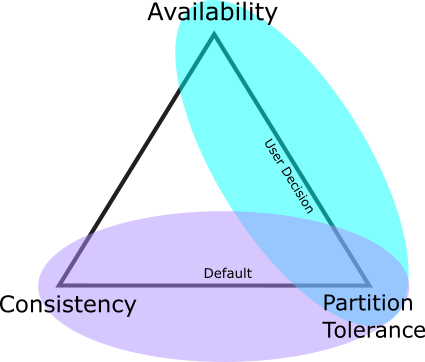
\includegraphics{img/rethinkCapTheorem.png}
    \caption{Overview of the CAP Theorem in RethinkDB}
    \label{fig:rethink_cap_theorem}
\end{figure}

\subsubsection{Performance}

In a test conducted by the RethinkDB core team the developers concluded that the database scales horizontally in a near linear fashion \autocite{rethinkdb:performance} as can be seen in \autoref{fig:rethink_rethink_performance}. The developers further imply that there will be ongoing efforts to improve upon this results.

\begin{figure}[ht]
    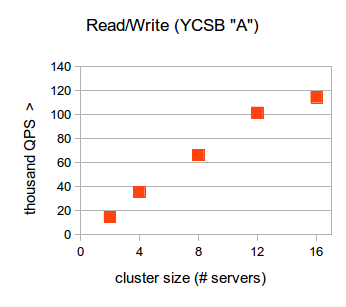
\includegraphics[width=.45\linewidth]{img/rethinkperf_rw.png} \quad
    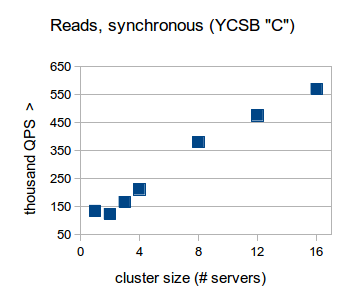
\includegraphics[width=0.45\linewidth]{img/rethinkperf_rsync.png}
    \\[\baselineskip]
    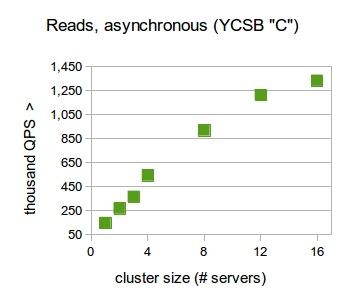
\includegraphics[width=0.45\linewidth]{img/rethinkperf_rasync.png} \quad
    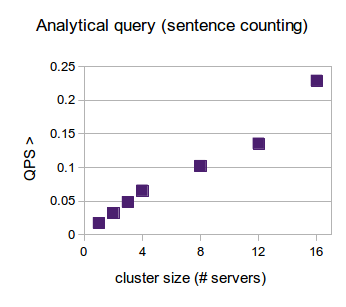
\includegraphics[width=0.45\linewidth]{img/rethinkperf_aquery.png}
    \caption{Overview of performance test results\autocite{rethinkdb:performance}}
    \label{fig:rethink_rethink_performance}
\end{figure}

\subsubsection{Comparison to real-time sync APIs}
The functionality of RethinkDB can be compared to many real-time sync API services like Pusher\footnote{https://pusher.com} or Firebase\footnote{https://firebase.google.com/products/realtime-database/}. There are some key differences between those kinds of systems and RethinkDB.

The capability to store information is the most noticeable difference. Sync APIs don't store any data. They are intended to send uniform event streams to a large amount of recipients. Other key differences can be taken from \autoref{tbl:rethink_realtimesync}.

\begin{table}[ht]
\caption{Comparison of RethinkDB and real-time sync APIs}
\label{tbl:rethink_realtimesync}
\centering
\begin{tabular}{|p{0.55\textwidth}|p{0.34\textwidth}|}
\hline
RethinkDB & Real-time sync APIs \\ \hline
Open source 
\newline
$\rightarrow$ Can be deployed on any infrastructure
&
Cloud Service \\ \hline
General Purpose Database System \newline
$\rightarrow$ Can run complex queries
&
Syncing documents
$\rightarrow$ limited querying\\ \hline
Designed to be accessed from an application server\newline
$\rightarrow$ More complex to set up \newline
$\rightarrow$ More flexible \newline
$\rightarrow$ Works for sophisticated applications
&
Access directly over browser \newline
$\rightarrow$ Easy to setup \newline
$\rightarrow$ Limits flexibility\\
\hline
\end{tabular}
\end{table}

\subsubsection{Use Cases}
RethinkDB is useful in any situation where data needs to be stored and distributed at the same time\autocite{rethinkdb:faq}. The following list contains major use cases for the database.

\begin{itemize}
    \item Collaborative web and mobile apps
    \item Streaming analytics apps
    \item Multiplayer games
    \item Real-time marketplaces
    \item Connected devices
\end{itemize}
There are some use cases RethinkDB should not be applied to, gathered in the following list.

\begin{itemize}
    \item Applications that need full ACID support
    \item Strong schema enforcement is required
    \item Computationally intensive analytics
    \item High write availability is critical
\end{itemize}

\subsubsection{Conclusion}

Working with RethinkDB we found the documentation to be extraordinarily comprehensive. Every major feature could be found described in great detail and supported by multiple examples. Nevertheless there is some confusion concerning the term of real-time databases, since many different definitions exist. This made it harder to evaluate the topic in general and specifically in connection with RethinkDB. This was complicated even further by the fact that RethinkDB in fact 'rethought' databases, delivering a product that can hardly be forced into predefined categories.

However, due to this impossibility to classify the database, RethinkDB was very refreshing to work with, providing many new features and combining the advantages of multiple different database types.

Working with the Database proved to be very convenient. The documentation made it easy to get used to the specifics of RethinkDB. We had no chance to use all the features ReQL gives the user, due to it having to many and specialised features. We also were not able to test the software in a cluster configuration. Therefore testing the behaviour with sharding and replication setting applied was not possible.

In general we found RethinkDB very useful and where able to identify fitting use cases while testing the database.

We think that not only real-time databases but also RethinkDB will become more and more important in the near future, with big data and IoT redefining the world of databases. 
